\chapter{Sequential Logic Circuits}\label{ch09}
\section{Introduction}

Electronic circuits that require memory devices (like flip-flops or registers) and feedback loops are designed using is called ``Sequential Logic.'' The final output of the circuit is determined by both the inputs and internal circuit feedback loops; and the states of the various logic gates may change rapidly as the output from one stage is fed back to various input points. This makes sequential logic circuits much more dynamic, and complex, than combinational circuits, and their analysis normally requires tools like timing diagrams and state maps. Because sequential circuits are able to latch and hold output states, useful applications like flip-flops, registers, counters, and memory are possible.

%***************************************************************************
% Section: Timing Diagrams
%***************************************************************************
\section{Timing Diagrams}
\label{SL:sec:timing_diagrams}

Unlike combinational logic circuits, timing is essential in sequential circuits. Normally, a device will include a \emph{clock} \ac{IC} that generates a square wave that is used to control the sequencing of various activities throughout the device. In order to design and troubleshoot these types of circuits, a timing diagram is developed that shows the relationship between the various input, intermediate, and output signals. Figure \ref{tmg:09_01} is an example timing diagram.

\begin{figure}[H]
  \centering
  \begin{tikztimingtable}[
        timing/slope=0,         % no slope
        timing/coldist=2pt,     % column distance
        xscale=2.0,yscale=1.0,  % scale diagrams
        semithick,               % set line width
    ]
    \footnotesize \# & U     R 8{2Q} 2U     \\
    \footnotesize Clk & 17{C} \\
    %                      P 01 02 03 04 05 06 07 08
    \footnotesize In & [] {L HH LH HL LL LH LL HL HL} \\
    \footnotesize Out & []{L HH LL HH LL LL LL HH HH} \\
    \extracode % Optional
    % \fulltablegrid[]
    % \vertlines[]{}
    \tablerules[]
  \end{tikztimingtable}
  \caption{Example Timing Diagram} 
  \label{tmg:09_01}
\end{figure}

Figure \ref{tmg:09_01} is a timing diagram for a device that has three signals, a clock, an Input, and an Output. 

\begin{itemize}
  \marginpar{Signals in a timing diagram can be described as low//high, $ 0 $//$ 1 $, on//off, or any other number of ways.}

  \item \textsc{\#}: The first line of the timing diagram is only a counter that indicates the number of times the system clock has cycled from Low to High and back again. For example, the first time the clock changes from Low to High is the beginning of the first cycle. This counter is only used to facilitate a discussion about the circuit timing. 

  \item \textsc{Clk}: A clock signal regularly varies between Low and High in a predictable pattern, normally such that the amount of Low time is the same as the High time. In a circuit, a clock pulse is frequently generated by applying voltage to a crystal since the oscillation cycle of a crystal is well known and extremely stable. In Figure \ref{tmg:09_01} the clock cycle is said have a $ 50 $\% duty cycle, that is, half-low and half-high. The exact length of a single cycle would be measured in micro- or nano-seconds but for the purposes of this book all that matters is the relationship between the various signals, not the specific length of a clock cycle.
  
  \item \textsc{In}: The input is Low until Cycle \#$ 1 $, then goes High for one cycle. It then toggles between High and Low at irregular intervals.
  
  \item \textsc{Out}: The output goes High at the beginning of cycle \#$ 1 $. It then follows the input, but only at the start of a clock cycle. Notice that the input goes high halfway through cycle \#$ 2 $ but the output does not go high until the start of cycle \#$ 3 $. Most devices are manufactured to be \emph{edge triggered} and will only change their output at either the positive or negative edge of the clock cycle (this example is positive edge triggered). Thus, notice that no matter when the input toggles the output only changes when the clock transitions from Low to High.

\end{itemize}

Given the timing diagram in Figure \ref{tmg:09_01} it would be relatively easy to build a circuit to match the timing requirements. It would have a single input and output port and the output would match the input on the positive edge of a clock cycle.

Whenever the input for any device changes it takes a tiny, but measurable, amount of time for the output to change since the various transistors, capacitors, and other electronic elements must reach saturation and begin to conduct current. This lag in response is known as \emph{propagation delay} and that is important for an engineer to consider when building a circuit. \marginpar{Ideal circuits with no propagation delay are assumed in this book in order to focus on digital logic rather than engineering.} It is possible to have a circuit that is so complex that the output has still not changed from a previous input signal before a new input signal arrives and starts the process over. In Figure \ref{tmg:09_02} notice that the output goes High when the input goes Low, but only after a tiny propagation delay. 

\begin{figure}[H]
  \centering
  \begin{tikztimingtable}[
    timing/slope=0,         % no slope
    timing/coldist=2pt,     % column distance
    xscale=2.0,yscale=1.0,  % scale diagrams
    semithick,               % set line width
    ]
    \footnotesize \# & U     R 8{2Q} 2U     \\
    \footnotesize Clk & 17{C} \\
    %                      P 01 02 03 04 05 06 07 08
    \footnotesize In & [] {L 2L 1H 2L 1H 2L 1H 2L 1H 2L 1H 1L} \\
    \footnotesize Out & []{L 3.25L 0.75H 2.25L 0.75H 
                            2.25L 0.75H 2.25L 0.75H 2.25L .75H} \\
    \extracode % Optional
    % \fulltablegrid[]
    % \vertlines[]{}
    \tablerules[]
  \end{tikztimingtable}
  \caption{Example Propagation Delay} 
  \label{tmg:09_02}
\end{figure}

It is also true that a square wave is not exactly square. Due to the presence of capacitors and inductors in circuits, a square wave will actually build up and decay over time rather than instantly change. Figure \ref{drw:09_01} shows a typical charge/discharge cycle for a capacitance circuit and the resulting deformation of a square wave. It should be kept in mind, though, that the times involved for capacitance charge/discharge are quite small (measured in nanoseconds or smaller); so for all but the most sensitive of applications, square waves are assumed to be truly square.

\begin{figure}[H]
  \myfloatalign
  \begin{tikzpicture} [circuit logic US, scale=0.50]
  % make all path lines (the node shapes) a little thicker
  \tikzstyle{every path}=[line width=0.50mm]  
  
  % Draw the lines
  \draw[gray,thin] (0,0) grid [step=4] (20,4);
  \draw 
    (0,4) .. controls ( 0.05,0.50) and ( 0.50,0.05) .. (4,0)
          .. controls ( 4.05,3.50) and ( 4.55,3.95) .. (8,4)
          .. controls ( 8.05,0.50) and ( 8.50,0.05) .. (12,0)
          .. controls (12.05,3.50) and (12.55,3.95) .. (16,4)
          .. controls (16.05,0.50) and (16.50,0.05) .. (20,0)
  ;
  \end{tikzpicture}
  \caption{Capacitor Charge and Discharge}
	\label{drw:09_01}  
\end{figure}

All devices are manufactured with certain tolerance levels built-in such that when the voltage gets ``close'' to the required level then the device will react, thus mitigating the effect of the deformed square wave. Also, for applications where speed is critical, such as space exploration or medical, high-speed devices are available that both sharpen the edges of the square wave and reduce propagation delay significantly. 

%***************************************************************************
% Section: Flip-Flops
%***************************************************************************
\section{Flip-Flops}
\label{SL:sec:flip-flops}

\subsection{Introduction}
\label{SL:subsec:intro_to_flip-flops}

Flip-flops are digital circuits that can maintain an electronic state even after the initial signal is removed. They are, then, the simplest of memory devices. Flip-flops are often called \emph{latches} since they are able to ``latch'' and hold some electronic state. In general, devices are called flip-flops when sequential logic is used and the output only changes on a clock pulse and they are called latches when combinational logic is used and the output constantly reacts to the input. Commonly, flip-flops are used for clocked devices, like counters, while latches are used for storage. However, these terms are often considered synonymous and are used interchangeably.

\subsection{SR Latch}
\label{SL:subsec:sr_latch}

One of the simplest of the flip-flops is the SR (for \emph{Set-Reset}) latch. \marginpar{This latch is often also called an \emph{RS Latch}.} Figure \ref{fig:09_01} illustrates a logic diagram for an \emph{SR latch} built with \textsf{NAND} gates.

\begin{figure}[H]
	\centering
	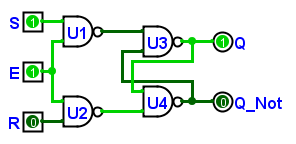
\includegraphics[width=\maxwidth{.95\linewidth}]{gfx/09_01}
	\caption{SR Latch Using NAND Gates}
	\label{fig:09_01}
\end{figure}

Table \ref{tab:09_01} is the truth table for an \emph{SR Latch}. Notice that unlike truth tables used earlier in this book, some of the outputs are listed as ``Last Q'' since they do not change from the previous state.

\begin{table}[H]
  \sffamily
  \newcommand{\head}[1]{\textcolor{white}{\textbf{#1}}}    
  \begin{center}
    \rowcolors{2}{gray!10}{white} % Color every other line a light gray
    \begin{tabular}{ccccc} 
      \rowcolor{black!75}
      \multicolumn{3}{c}{\head{Inputs}} & \multicolumn{2}{c}{\head{Outputs}} \\
      E & S & R & Q & Q' \\
      \hline
      0 & 0 & 0 & Last Q & Last Q' \\
      0 & 0 & 1 & Last Q & Last Q' \\
      0 & 1 & 0 & Last Q & Last Q' \\
      0 & 1 & 1 & Last Q & Last Q' \\
      1 & 0 & 0 & Last Q & Last Q' \\
      1 & 0 & 1 & 0 & 1 \\
      1 & 1 & 0 & 1 & 0 \\
      1 & 1 & 1 & Not Allowed & Not Allowed \\
    \end{tabular}
  \end{center}
  \caption{Truth Table for SR Latch}
  \label{tab:09_01}
\end{table}

In Figure \ref{fig:09_01}, input \emph{E} is an enable and must be high for the latch to work; when it is low then the output state remains constant regardless of how inputs \emph{S} or \emph{R} change. When the latch is enabled, if $ S=R=0 $ then the values of \emph{Q} and \emph{Q'} remain fixed at their last value; or, the circuit is ``remembering'' how they were previously set. When input \emph{S} goes high, then \emph{Q} goes high (the latch's output, \emph{Q}, is ``set''). When input \emph{R} goes high, then \emph{Q'} goes high (the latch's output, \emph{Q}, is ``reset''). Finally, it is important that in this latch inputs \emph{R} and \emph{S} cannot both be high when the latch is enabled or the circuit becomes unstable and output \emph{Q} will oscillate between high and low as fast as the \textsf{NAND} gates can change; thus, input $ 111_2 $ must be avoided. Normally, there is an additional bit of circuit prior to the inputs to ensure \emph{S} and \emph{R} will always be different (an \textsf{XOR} gate could do that job).

An SR Latch may or may not include a clock input; if not, then the outputs change immediately when any of the inputs change, like in a combinational circuit. If the designer needs a clocked type of memory device, which is routine, then the typical choice would be a \emph{JK Flip-Flop}, covered later. Figure \ref{tmg:09_03} is a timing diagram for the SR Latch in Listing \ref{fig:09_01}.

\begin{figure}[H]
  \centering
  \begin{tikztimingtable}[
    timing/slope=0,         % no slope
    timing/coldist=2pt,     % column distance
    xscale=2.0,yscale=1.0,  % scale diagrams
    semithick,               % set line width
    ]
    \footnotesize \# & U     R 8{2Q} 2U     \\
%    \footnotesize Clk & 17{C} \\
    %                        P 01 02 03 04 05 06 07 08
    \footnotesize Ena  & [] {L LL LL HH HH HH HH HH HH} \\
    \footnotesize S    & [] {H HH LL HH LL LL HH HH HH} \\
    \footnotesize R    & [] {L LL HH LL LL HH HH LL LL} \\
    \footnotesize Q    & [] {H HH HH HH HH LL LL HH HH} \\
    \footnotesize Qn   & [] {L LL LL LL LL HH LL LL LL} \\
    \extracode % Optional
    % \fulltablegrid[]
    % \vertlines[]{}
    \tablerules[]
  \end{tikztimingtable}
  \caption{SR Latch Timing Diagram} 
  \label{tmg:09_03}
\end{figure}

At the start of Figure \ref{tmg:09_03} \emph{Enable} is low and there is no change in $ Q $ and $ Q' $ until frame 3, when \emph{Enable} goes high. At that point, $ S $ is high and $ R $ is low so $ Q $ is high and $ Q' $ is low. At frame $ 4 $ both $ S $ and $ R $ are low so there is no change in $ Q $ or $ Q' $. At frame 5 $ R $ goes high so $ Q $ goes low and $ Q' $ goes high. In frame $ 6 $ both $ S $ and $ R $ are high so both $ Q $ and $ Q' $ go low. Finally, in frame $ 7 $ $ S $ stays high and $ R $ goes low so $ Q $ goes high and $ Q' $ stays low.

\Le includes an \emph{S-R Flip-Flop} device, as illustrated in Figure \ref{fig:09_02}. 

\begin{figure}[H]
	\centering
	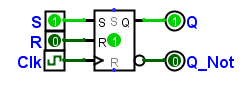
\includegraphics[width=\maxwidth{.95\linewidth}]{gfx/09_02}
	\caption{SR Latch}
	\label{fig:09_02}
\end{figure}

The \emph{S-R Flip-Flop} has \emph{S} and \emph{R} input ports and \emph{Q} and \emph{Q'} output ports. Also notice that there is no \emph{Enable} input but there is a \emph{Clock} input.\marginpar{On a logic diagram a clock input is indicated with a triangle symbol.} Because this is a clocked device the output would only change on the edge of a clock pulse and that makes the device a flip-flop rather than a latch. As shown, \emph{S} is high and the clock has pulsed so \emph{Q} is high, or the flip-flop is ``set.'' Also notice that on the top and bottom of the device there is an \emph{S} and \emph{R} input port that are not connected. These are ``preset'' inputs that let the designer hard-set output \emph{Q} at either one or zero, which is useful during a power-up routine. Since this device has no \emph{Enable} input it is possible to use the \emph{R} preset port as a type of enable. If a high is present on the \emph{R} preset then output \emph{Q} will go low and stay there until the \emph{R} preset returns to a low state.

\subsection{Data (D) Flip-Flop}
\label{SL:subsec:data_latch}

A Data Flip-Flop (or \emph{D Flip-Flop}) is formed when the inputs for an \emph{SR Flip-Flop} are tied together through an inverter (which also means that \emph{S} and \emph{R} cannot be high at the same time, which corrects the potential problem with two high inputs in an \emph{SR Flip-Flop}). Figure \ref{fig:09_03} illustrates an \emph{SR Flip-Flop} being used as a \emph{D Flip-Flop} in \Le. 

\begin{figure}[H]
	\centering
	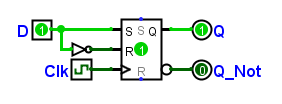
\includegraphics[width=\maxwidth{.95\linewidth}]{gfx/09_03}
	\caption{D Flip-Flop Using SR Flip-Flop}
	\label{fig:09_03}
\end{figure}

In Figure \ref{fig:09_03}, the \emph{D} input (for ``Data'') is latched and held on each clock cycle. Even though Figure \ref{fig:09_03} shows the inverter external to the latch circuit, in reality, a \emph{D Flip-Flop} device bundles everything into a single package with only \emph{D} and clock inputs and \emph{Q} and \emph{Q'} outputs, as in Figure \ref{fig:09_04}. Like the \emph{RS Flip-Flop}, \emph{D Flip-Flops} also have ``preset'' inputs on the top and bottom that lets the designer hard-set output \emph{Q} at either one or zero, which is useful during a power-up routine.

\begin{figure}[H]
	\centering
	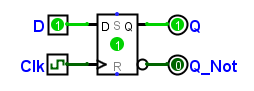
\includegraphics[width=\maxwidth{.95\linewidth}]{gfx/09_04}
	\caption{D Flip-Flop}
	\label{fig:09_04}
\end{figure}

Figure \ref{tmg:09_04} is the timing diagram for a Data Flip-Flop.

\begin{figure}[H]
  \centering
  \begin{tikztimingtable}[
    timing/slope=0,         % no slope
    timing/coldist=2pt,     % column distance
    xscale=2.0,yscale=1.0,  % scale diagrams
    semithick,               % set line width
    ]
    \footnotesize \# & U     R 8{2Q} 2U     \\
%    \footnotesize Clk & 17{C} \\
    %                     P 01 02 03 04 05 06 07 08
    \footnotesize Clk & [] {L HL HL HL HL HL HL HL HL} \\
    \footnotesize D & []   {H HH LL HH LL HL HH LH HH} \\
    \footnotesize Q & []   {H HH LL HH LL HH HH LL HH} \\
    \extracode % Optional
    % \fulltablegrid[]
    % \vertlines[]{}
    \tablerules[]
  \end{tikztimingtable}
  \caption{D Latch Timing Diagram} 
  \label{tmg:09_04}
\end{figure}

In Figure \ref{tmg:09_04} it is evident that output \emph{Q} follows input \emph{D} but only on a positive clock edge. The latch ``remembers'' the value of \emph{D} until the next clock pulse no matter how it changes between pulses. 

\subsection{JK Flip-Flop}
\label{SL:subsec:jk_flip-flop}

The \emph{JK flip-flop} is the ``workhorse'' of the flip-flop family. Figure \ref{fig:09_05} is the logic diagram for a \emph{JK flip-flop}.

\begin{figure}[H]
	\centering
	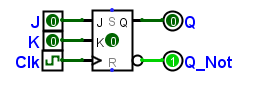
\includegraphics[width=\maxwidth{.95\linewidth}]{gfx/09_05}
	\caption{JK Flip-Flop}
	\label{fig:09_05}
\end{figure}

Internally, a \emph{JK flip-flop} is similar to an \emph{RS Latch}. However, the outputs to the circuit (\emph{Q} and \emph{Q'}) are connected to the inputs (\emph{J} and \emph{K}) in such a way that the unstable input condition (both \emph{R} and \emph{S} high) of the \emph{RS Latch} is corrected. If both inputs, \emph{J} and \emph{K}, are high then the outputs are toggled (they are ``flip-flopped'') on the next clock pulse. This toggle feature makes the \emph{JK flip-flop} extremely useful in many logic circuits.

Figure \ref{tmg:09_05} is the timing diagram for a \emph{JK flip-flop}.

\begin{figure}[H]
  \centering
  \begin{tikztimingtable}[
    timing/slope=0,         % no slope
    timing/coldist=2pt,     % column distance
    xscale=2.0,yscale=1.0,  % scale diagrams
    semithick,               % set line width
    ]
    \footnotesize \# & U     R 8{2Q} 2U     \\
    \footnotesize Clk & 17{C} \\
    %                      P 01 02 03 04 05 06 07 08
    \footnotesize J  & [] {H HH LL LL LL HL LL LL LL} \\
    \footnotesize K  & [] {L LL HH HH LL HL LL HH LL} \\
    \footnotesize Q  & [] {H HH LL LL LL HH HH LL LL} \\
    \footnotesize Q' & [] {L LL HH HH HH LL LL HH HH} \\
    \extracode % Optional
    % \fulltablegrid[]
    % \vertlines[]{}
    \tablerules[]
  \end{tikztimingtable}
  \caption{JK Flip-Flop Timing Diagram} 
  \label{tmg:09_05}
\end{figure}

Table \ref{tab:09_01} summarizes timing diagram \ref{tmg:09_05}. Notice that on clock pulse five both \emph{J} and \emph{K} are high so \emph{Q} toggles. Also notice that \emph{Q'} is not indicated in the table since it is always just the complement of \emph{Q}.

\begin{table}[H]
	\sffamily
	\newcommand{\head}[1]{\textcolor{white}{\textbf{#1}}}		
	\begin{center}
		\rowcolors{2}{gray!10}{white} % Color every other line a light gray
		\begin{tabular}{cccc} 
			\rowcolor{black!75}
			\head{Clock Pulse} & \head{J} & \head{K} & \head{Q} \\
			1 & H & L & H \\
			2 & L & H & L \\
			3 & L & H & L \\
			4 & L & L & L \\
			5 & H & H & H \\
			6 & L & L & H \\
			7 & L & H & L \\
			8 & L & L & L 
		\end{tabular}
	\end{center}
	\caption{JK Flip-Flop Timing Table}
	\label{tab:09_01}
\end{table}

\subsection{Toggle (T) Flip-Flop}
\label{SL:subsec:toggle_flip-flop}

If the J and K inputs to a \emph{JK Flip-Flop} are tied together, then when the input is high the output will toggle on every clock pulse but when the input is Low then the output remains in the previous state. This is often referred to as a \emph{Toggle Flip-Flop} (or \emph{T Flip-Flop}). \emph{T Flip-Flops} are not usually found in circuits as separate \acp{IC} since they are so easily created by soldering together the inputs of a standard \emph{JK Flip-Flop}. Figure \ref{fig:09_06} is a \emph{T Flip-Flop} in \Le.

\begin{figure}[H]
	\centering
	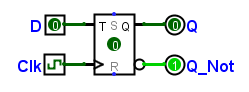
\includegraphics[width=\maxwidth{.95\linewidth}]{gfx/09_06}
	\caption{T Flip-Flop}
	\label{fig:09_06}
\end{figure}

Figure \ref{tmg:09_06} is the timing diagram for a \emph{T flip-flop}.

\begin{figure}[H]
  \centering
  \begin{tikztimingtable}[
    timing/slope=0,         % no slope
    timing/coldist=2pt,     % column distance
    xscale=2.0,yscale=1.0,  % scale diagrams
    semithick,               % set line width
    ]
    \footnotesize \# & U     R 8{2Q} 2U     \\
    \footnotesize Clk & 17{C} \\
    %                      P 01 02 03 04 05 06 07 08
    \footnotesize D  & [] {H HH HL LL LH HH HL LH HH} \\
    \footnotesize Q  & [] {H LL HH HH HH LL HH HH LL} \\
    \footnotesize Q' & [] {L HH LL LL LL HH LL LL HH} \\
    \extracode % Optional
    % \fulltablegrid[]
    % \vertlines[]{}
    \tablerules[]
  \end{tikztimingtable}
  \caption{Toggle Flip-Flop Timing Diagram} 
  \label{tmg:09_06}
\end{figure}

In Figure \ref{tmg:09_06} when \emph{D}, the data input, is high then \emph{Q} toggles on the positive edge of every clock cycle.

\subsection{Master-Slave Flip-Flops}
\label{SL:subsec:master-slave_flip-flops}

Master-Slave Flip-Flops are two flip-flops connected in a cascade and operating from the same clock pulse. These flip-flops tend to stabilize an input circuit and are used where the inputs may have voltage glitches (such as from a push button). Figure \ref{fig:09_07} is the logic diagram for two \emph{JK flip-flops} set up as a Master-Slave Flip-Flop.

\begin{figure}[H]
	\centering
	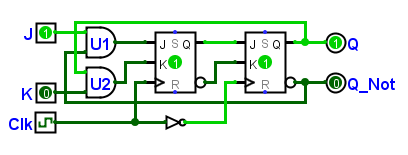
\includegraphics[width=\maxwidth{.95\linewidth}]{gfx/09_07}
	\caption{Master-Slave Flip-Flop}
	\label{fig:09_07}
\end{figure}

Because of the \textsf{NOT} gate on the clock signal these two flip-flops will activate on opposite clock pulses, which means the flip-flop one will enable first and read the JK inputs, then flip-flop two will enable and read the output of flip-flop one. The result is that any glitches on the input signals will tend to be eliminated.

Often, only one physical \ac{IC} is needed to provide the two flip-flops for a master-slave circuit because dual \emph{JK flip-flops} are frequently found on a single \ac{IC}. Thus, the output pins for one flip-flop could be connected directly to the input pins for the second flip-flop on the same \ac{IC}. By combining two flip-flops into a single \ac{IC} package, circuit design can be simplified and fewer components need to be purchased and mounted on a circuit board. 

%***************************************************************************
% Section: Registers
%***************************************************************************
\section{Registers}
\label{SL:sec:registers}

\subsection{Introduction}
\label{SL:subsec:intro_to_registers}

A register is a simple memory device that is composed of a series of flip-flops wired together such that they share a common clock pulse. Registers come in various sizes and types and are often used as ``scratch pads'' for devices. For example, a register can hold a number entered on a keypad until the calculation circuit is ready do something with that number or a register can hold a byte of data coming from a hard drive until the \ac{CPU} is ready to move that data someplace else. 

\subsection{Registers As Memory}
\label{SL:subsec:registers_as_memory}

Internally, a register is constructed from \emph{D Flip-Flops} as illustrated in Figure \ref{fig:09_08}.

\begin{figure}[H]
	\centering
	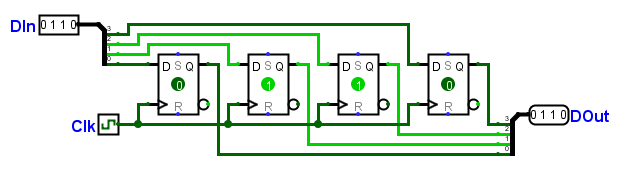
\includegraphics[width=\maxwidth{.95\linewidth}]{gfx/09_08}
	\caption{4-Bit Register}
	\label{fig:09_08}
\end{figure}

Data are moved from the input port, in the upper left corner, into the register; one bit goes into each of the four \emph{D Flip-Flops}. Because each latch constantly outputs whatever it contains, the output port, in the lower right corner, combines the four data bits and displays the contents of the register. Thus, a four-bit register can ``remember'' some number until it is needed, it is a four-bit memory device.

\subsubsection{74x273 Eight-Bit Register}
\label{SL:subsubsec:74x273_8-bit_register}

In reality, designers do not build memory from independent flip-flops, as shown in Figure \ref{fig:09_08}. Instead, they use a memory \ac{IC} that contains the amount of memory needed. In general, purchasing a memory \ac{IC} is cheaper and more reliable than attempting to build a memory device.

One such memory device is a $ 74x273 $ eight-bit register. This device is designed to load and store a single eight-bit number, but other memory devices are much larger, including \ac{RAM} that can store and retrieve millions of eight-bit bytes.

\subsection{Shift Registers}
\label{SL:subsec:shift_registers}

Registers have an important function in changing a stream of data from serial to parallel or parallel to serial; a function that is called ``shifting'' data. For example, data entering a computer from a network or \ac{USB} port is in serial form; that is, one bit at a time is streamed into or out of the computer. However, data inside the computer are always moved in parallel; that is, all of the bits in a word are placed on a bus and moved through the system simultaneously. Changing data from serial to parallel or vice-verse is an essential function and enables a computer to communicate over a serial device.

Figure \ref{fig:09_09} illustrates a four-bit parallel-in/serial-out shift register. The four-bit data into the register is placed on \emph{D0}-\emph{D3}, the \emph{Shift\_Write} bit is set to $ 1 $ and the clock is pulsed to write the data into the register. Then the \emph{Shift\_Write} bit is set to $ 0 $ and on each clock pulse the four bits are shifted right to the \emph{SOUT} (for ``serial out'') port.

\begin{figure}[H]
	\centering
	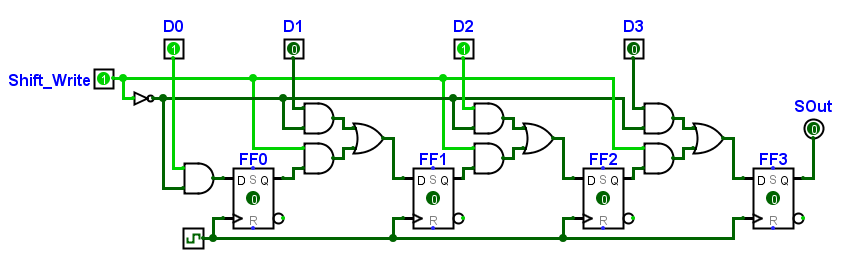
\includegraphics[width=\maxwidth{.95\linewidth}]{gfx/09_09}
	\caption{Shift Register}
	\label{fig:09_09}
\end{figure}

It is possible to also build other shift register configurations: serial-in/serial-out, parallel-in/parallel-out, and serial-in/parallel-out. However, universal shift registers are commonly used since they can be easily configured to work with data in either serial or parallel formats.

%***************************************************************************
% Section: Counters
%***************************************************************************
\section{Counters}
\label{SL:sec:counters}

\subsection{Introduction}
\label{SL:subsec:intro_to_counters}

Counters are a type of sequential circuit designed to count input pulses (normally from a clock) and then activate some output when a specific count is reached. Counters are commonly used as timers; thus, all digital clocks, microwave ovens, and other digital timing displays use some sort of counting circuit. However, counters can be used in many diverse applications. For example, a speed gauge is a counter. By attaching some sort of sensor to a rotating shaft and counting the number of revolutions for $ 60 $ seconds the \ac{RPM} is determined. Counters are also commonly used as frequency dividers. If a high frequency is applied to the input of a counter, but only the ``tens'' count is output, then the input frequency will be divided by ten. As one final example, counters can also be used to control sequential circuits or processes; each count can either activate or deactivate some part of a circuit that controls one of the sequential processes. 

\subsection{Asynchronous Counters}
\label{SL:subsec:asynchronous_counters}

One of the simplest counters possible is an asynchronous two-bit counter. This can be built with a two \emph{JK flip-flops} in sequence, as shown in Figure \ref{fig:09_10}.

\begin{figure}[H]
	\centering
	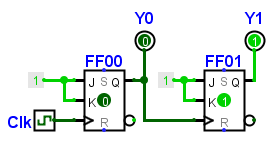
\includegraphics[width=\maxwidth{.95\linewidth}]{gfx/09_10}
	\caption{Asynchronous 2-Bit Counter}
	\label{fig:09_10}
\end{figure}

The J-K inputs on both flip-flops are tied high and the clock is wired into \emph{FF00}. On every positive-going clock pulse the \emph{Q} output for \emph{FF00} toggles and that is wired to the clock input of \emph{FF01}, toggling that output. This type of circuit is frequently called a ``ripple'' counter since the clock pulse must ripple through all of the flip-flops.

In Figure \ref{fig:09_10}, assume both flip-flops start with the output low (or $ 00 $ out). On the first clock pulse, \emph{Q\_FF00} will go high, and that will send a high signal to the clock input of \emph{FF01} which activates \emph{Q\_FF01}. At this point, the \emph{Q} outputs for both flip-flops are high (or $ 11 $ out). On the next clock pulse, \emph{Q\_FF00} will go low, but \emph{Q\_FF01} will not change since it only toggles when the clock goes from low to high. At this point, the output is $ 01 $. On the next clock pulse, \emph{Q\_FF00} will go high and \emph{Q\_FF01} will toggle low: $ 10 $. The next clock pulse toggles \emph{Q\_FF00} to low but \emph{Q\_FF01} does not change: $ 00 $. Then the cycle repeats. This simple circuit counts: $ 00 $, $ 11 $, $ 10 $, $ 01 $. (Note, \emph{Q\_FF00} is the low-order bit.) This counter is counting backwards, but it is a trivial exercise to add the functionality needed to reverse that count.

An asynchronous three-bit counter looks much like the asynchronous two-bit counter, except that a third stage is added.

\begin{figure}[H]
	\centering
	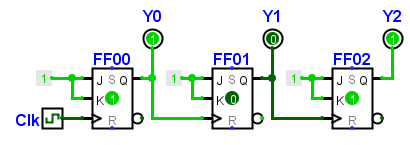
\includegraphics[width=\maxwidth{.95\linewidth}]{gfx/09_11}
	\caption{Asynchronous 3-Bit Counter}
	\label{fig:09_11}
\end{figure}

In Figure \ref{fig:09_11}, the ripple of the clock pulse from one flip-flop to the next is more evident than in the two-bit counter. However, the overall operation of this counter is very similar to the two-bit counter.

More stages can be added so to any desired number of outputs. Asynchronous (or ripple) counters are very easy to build and require very few parts. Unfortunately, they suffer from two rather important flaws:

\begin{itemize}
  \item \textsc{Propagation Delay}. As the clock pulse ripples through the various flip-flops, it is slightly delayed by each due to the simple physical switching of the circuitry within the flip-flop. Propagation delay cannot be prevented and as the number of stages increases the delay becomes more pronounced. At some point, one clock pulse will still be winding its way through all of the flip-flops when the next clock pulse hits the first stage and this makes the counter unstable. 

  \item \textsc{Glitches}. If a three-bit counter is needed, there will be a very brief moment while the clock pulse ripples through the flip-flops that the output will be wrong. For example, the circuit should go from $ 111 $ to $ 000 $, but it will actually go from $ 111 $ to $ 110 $ then $ 100 $ then $ 000 $ as the ``low'' ripples through the flip-flops. These glitches are very short, but they may be enough to introduce errors into a circuit.
\end{itemize}

Figure \ref{fig:09_12} is a four-bit asynchronous counter.

\begin{figure}[H]
	\centering
	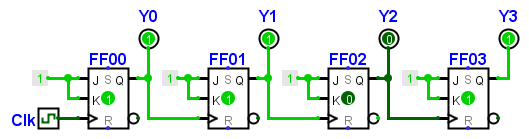
\includegraphics[width=\maxwidth{.95\linewidth}]{gfx/09_12}
	\caption{Asynchronous 4-Bit Counter}
	\label{fig:09_12}
\end{figure}

Figure \ref{tmg:09_07} is the timing diagram obtained when the counter in Figure \ref{fig:09_12} is executing.

\begin{figure}[H]
  \centering
  \begin{tikztimingtable}[
    timing/slope=0,         % no slope
    timing/coldist=2pt,     % column distance
    xscale=1.0,yscale=1.0,  % scale diagrams
    semithick,               % set line width
    ]
    \footnotesize \# & U     R 18{2Q} 2U     \\
    \footnotesize Clk & 36{C} \\
    %                      P 01 02 03 04 05 06 07 08 09 10 11 12 13 14 15 16 17 18
    \footnotesize Y0 & [] {L HH LL HH LL HH LL HH LL HH LL HH LL HH LL HH LL HH LL} \\
    \footnotesize Y1 & [] {L HH HH LL LL HH HH LL LL HH HH LL LL HH HH LL LL HH HH} \\
    \footnotesize Y2 & [] {L HH HH HH HH LL LL LL LL HH HH HH HH LL LL LL LL HH HH} \\
    \footnotesize Y3 & [] {L HH HH HH HH HH HH HH HH LL LL LL LL LL LL LL LL HH HH} \\
    \extracode % Optional
    % \fulltablegrid[]
    % \vertlines[]{}
    \tablerules[]
  \end{tikztimingtable}
  \caption{4-Bit Asynchronous Counter Timing Diagram} 
  \label{tmg:09_07}
\end{figure}

Notice that \emph{Y0} counts at half the frequency of the clock and then \emph{Y1} counts at half that frequency and so forth. Each stage that is added will count at half the frequency of the previous stage.

\subsection{Synchronous Counters}
\label{SL:subsec:synchronous_counters}

Both problems with ripple counters can be corrected with a synchronous counter, where the same clock pulse is applied to every flip-flop at one time. Here is the logic diagram for a synchronous two-bit counter: 

\begin{figure}[H]
	\centering
	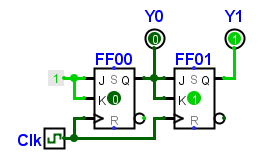
\includegraphics[width=\maxwidth{.95\linewidth}]{gfx/09_13}
	\caption{Synchronous 2-Bit Counter}
	\label{fig:09_13}
\end{figure}

Notice in this circuit, the clock is applied to both flip-flops and control is exercised by applying the output of one stage to both $ J $ and $ K $ inputs of the next stage, which effectively enables/disables that stage. When Q\_FF00 is high, for example, then the next clock pulse will make FF01 change states. 

\begin{figure}[H]
	\centering
	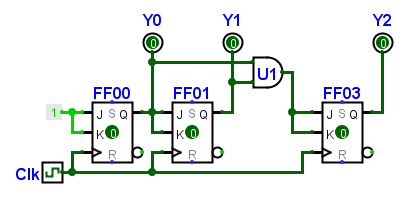
\includegraphics[width=\maxwidth{.95\linewidth}]{gfx/09_14}
	\caption{Synchronous 3-Bit Counter}
	\label{fig:09_14}
\end{figure}

A three-bit synchronous counter applies the clock pulse to each flip-flop. Notice, though, that the output from the first two stages must routed through an \textsf{AND} gate so \emph{FF03} will only change when \emph{Q\_FF00} and \emph{Q\_FF01} are high. This circuit would then count properly from $ 000 $ to $ 111 $. 

In general, synchronous counters become more complex as the number of stages increases since it must include logic for every stage to determine when that stage should activate. This complexity results in greater power usage (every additional gate requires power) and heat generation; however, synchronous counters do not have the propagation delay problems found in asynchronous counters. 

\begin{figure}[H]
	\centering
	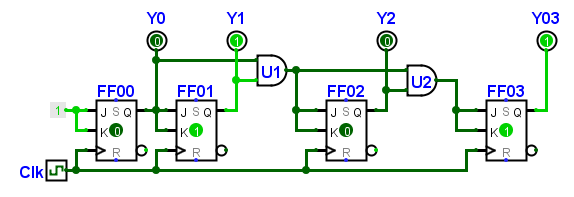
\includegraphics[width=\maxwidth{.95\linewidth}]{gfx/09_15}
	\caption{Synchronous 4-Bit Up Counter}
	\label{fig:09_15}
\end{figure}

Figure \ref{tmg:09_08} is the timing diagram for the circuit illustrated in Figure \ref{fig:09_15}.

\begin{figure}[H]
  \centering
  \begin{tikztimingtable}[
    timing/slope=0,         % no slope
    timing/coldist=2pt,     % column distance
    xscale=1.0,yscale=1.0,  % scale diagrams
    semithick,               % set line width
    ]
    \footnotesize \# & U     R 18{2Q} 2U     \\
    \footnotesize Clk & 36{C} \\
    %                      P 01 02 03 04 05 06 07 08 09 10 11 12 13 14 15 16
   %17 18
    \footnotesize Y0 & [] {L HH LL HH LL HH LL HH LL HH LL HH LL HH LL HH LL HH LL} \\
    \footnotesize Y1 & [] {L LL HH HH LL LL HH HH LL LL HH HH LL LL HH HH LL LL HH} \\
    \footnotesize Y2 & [] {L LL LL LL HH HH HH HH LL LL LL LL HH HH HH HH LL LL LL.} \\
    \footnotesize Y3 & [] {L LL LL LL LL LL LL LL HH HH HH HH HH HH HH HH LL LL LL} \\
    \extracode % Optional
    % \fulltablegrid[]
    % \vertlines[]{}
    \tablerules[]
  \end{tikztimingtable}
  \caption{4-Bit Synchronous Counter Timing Diagram} 
  \label{tmg:09_08}
\end{figure}

The timing diagram for the asynchronous counter in Figure \ref{tmg:09_07} is the same as that for an synchronous counter in Figure \ref{tmg:09_08} since the output of the two counters are identical. The only difference in the counters is in how the count is obtained, and designers would normally opt for a synchronous \ac{IC} since that is a more efficient circuit.

\subsubsection{Synchronous Down Counters}
\label{SL:subsubsec:synchronous_down_counters}

It is possible to create a counter that counts down rather than up by using the \emph{Q'} outputs of the flip-flops to trigger the next stage. Figure \ref{fig:09_16} illustrates a four-bit down counter.

\begin{figure}[H]
	\centering
	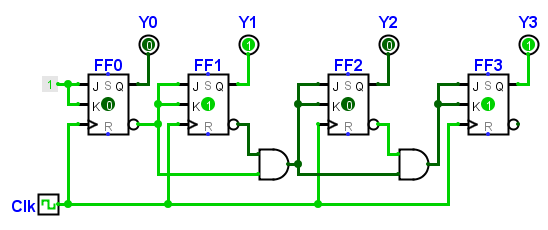
\includegraphics[width=\maxwidth{.95\linewidth}]{gfx/09_16}
	\caption{Synchronous 4-Bit Down Counter}
	\label{fig:09_16}
\end{figure}

Figure \ref{tmg:09_09} is the timing diagram for the circuit illustrated in Figure \ref{fig:09_16}.

\begin{figure}[H]
	\centering
	\begin{tikztimingtable}[
		timing/slope=0,         % no slope
		timing/coldist=2pt,     % column distance
		xscale=1.0,yscale=1.0,  % scale diagrams
		semithick,               % set line width
		]
		\footnotesize \# & U     R 18{2Q} 2U     \\
		\footnotesize Clk & 36{C} \\
		%                      P 01 02 03 04 05 06 07 08 09 10 11 12 13 14 15 16
	 %17 18
		\footnotesize Y0 & [] {L HH LL HH LL HH LL HH LL HH LL HH LL HH LL HH LL HH LL} \\
		\footnotesize Y1 & [] {L HH HH LL LL HH HH LL LL HH HH LL LL HH HH LL LL HH HH} \\
		\footnotesize Y2 & [] {L HH HH HH HH LL LL LL LL HH HH HH HH LL LL LL LL HH HH} \\
		\footnotesize Y3 & [] {L HH HH HH HH HH HH HH HH LL LL LL LL LL LL LL LL HH HH} \\
		\extracode % Optional
		% \fulltablegrid[]
		% \vertlines[]{}
		\tablerules[]
	\end{tikztimingtable}
	\caption{4-Bit Synchronous Down Counter Timing Diagram} 
	\label{tmg:09_09}
\end{figure}


\subsection{Ring Counters}
\label{SL:subsec:ring_counters}

A ring counter is a special kind of counter where only one output is active at a time. As an example, a four-bit ring counter may output this type of pattern:

\medskip
\texttt{ $ 1000 - 0100 - 0010 - 0001 $ }
\medskip

Notice the high output cycles through each of the bit positions and then recycles. Ring counters are useful as controllers for processes where one process must follow another in a sequential manner. Each of the bits from the ring counter can be used to activate a different part of the overall process; thus ensuring the process runs in proper sequence. The circuit illustrated in Figure \ref{fig:09_17} is a 4-bit ring counter.

\begin{figure}[H]
	\centering
	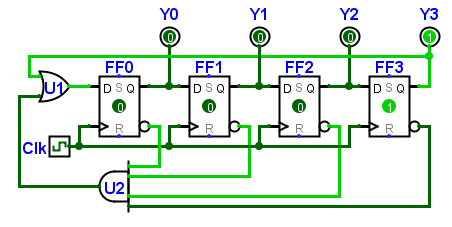
\includegraphics[width=\maxwidth{.95\linewidth}]{gfx/09_17}
	\caption{4-Bit Ring Counter}
	\label{fig:09_17}
\end{figure}

When the circuit is initialized none of the flip-flops are active. Because \emph{Q'} is high for all flip-flops, \textsf{AND} gate \emph{U2} is active and that sends a high through \emph{U1} and into the data port of \emph{FF0}. The purpose of \emph{U2} is to initialize \emph{FF0} for the first count and then \emph{U2} is never activated again. On each clock pulse the next flip-flop in sequence is activated. When \emph{FF3} is active that output is fed back through \emph{U1} to \emph{FF0}, completing the ring and re-starting the process.

Figure \ref{tmg:09_10} is the timing diagram for the ring counter illustrated in Figure \ref{fig:09_17}.

\begin{figure}[H]
  \centering
  \begin{tikztimingtable}[
    timing/slope=0,         % no slope
    timing/coldist=2pt,     % column distance
    xscale=2.0,yscale=1.0,  % scale diagrams
    semithick,               % set line width
    ]
    \footnotesize \# & U     R 8{2Q} 2U     \\
    \footnotesize Clk & 17{C} \\
    %                        P 01 02 03 04 05 06 07 08
    \footnotesize Y0 & [] {L HH LL LL LL HH LL LL LL} \\
    \footnotesize Y1 & [] {L LL HH LL LL LL HH LL LL} \\
    \footnotesize Y2 & [] {L LL LL HH LL LL LL HH LL} \\
    \footnotesize Y3 & [] {L LL LL LL HH LL LL LL HH} \\
    \extracode % Optional
    % \fulltablegrid[]
    % \vertlines[]{}
    \tablerules[]
  \end{tikztimingtable}
  \caption{4-Bit Ring Counter Timing Diagram} 
  \label{tmg:09_10}
\end{figure}

On each clock pulse a different bit is toggled high, proceeding around the four-bit nibble in a ring pattern.

\subsubsection{Johnson Counters}
\label{SL:subsubsec:johnson_counters}

One common modification of a ring counter is called a Johnson, or ``Twisted Tail,'' ring counter. In this case, the counter outputs this type of pattern.

\medskip
\texttt{ $ 1000 - 1100 - 1110 - 1111 - 0111 - 0011 - 0001 - 0000 $ }
\medskip

The circuit illustrated in Figure \ref{fig:09_18} is a 4-bit Johnson counter.

\begin{figure}[H]
	\centering
	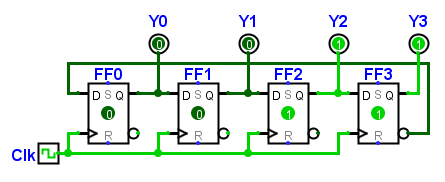
\includegraphics[width=\maxwidth{.95\linewidth}]{gfx/09_18}
	\caption{4-Bit Johnson Counter}
	\label{fig:09_18}
\end{figure}

This is very similar to the ring counter except the feedback loop is from \emph{Q'} rather than \emph{Q} of \emph{FF3} and because of that, the \textsf{AND} gate initialization is no longer needed. 

Figure \ref{tmg:09_11} is the timing diagram for the Johnson counter illustrated in Figure \ref{fig:09_18}.

\begin{figure}[H]
	\centering
	\begin{tikztimingtable}[
		timing/slope=0,         % no slope
		timing/coldist=2pt,     % column distance
		xscale=1.0,yscale=1.0,  % scale diagrams
		semithick,               % set line width
		]
		
    \footnotesize \# & U     R 18{2Q} 2U     \\
\footnotesize Clk & 36{C} \\
%                          P 01 02 03 04 05 06 07 08 09 10 11 12 13 14 15 16
%   17 18		
		\footnotesize Y0 & [] {L HH HH HH HH LL LL LL LL HH HH HH HH LL LL LL LL  HH H} \\
		\footnotesize Y1 & [] {L LL HH HH HH HH LL LL LL LL HH HH HH HH LL LL LL LL H} \\
		\footnotesize Y2 & [] {L LL LL HH HH HH HH LL LL LL LL HH HH HH HH LL LL LL L} \\
		\footnotesize Y3 & [] {L LL LL LL HH HH HH HH LL LL LL LL HH HH HH HH LL LL L} \\
		\extracode % Optional
		% \fulltablegrid[]
		% \vertlines[]{}
		\tablerules[]
	\end{tikztimingtable}
	\caption{4-Bit Johnson Counter Timing Diagram} 
	\label{tmg:09_11}
\end{figure}

\subsection{Modulus Counters}
\label{SL:subsec:modulus_counters}

Each of the counters created so far have had one significant flaw, they only count up to a number that is a power of two. A two-bit counter counts from zero to three, a three-bit counter counts from zero to seven, a four-bit counter counts from zero to $ 15 $, and so forth. With a bit more work a counter can be created that stops at some other number. These types of counters are called ``modulus counters'' and an example of one of the most common modulus counters is a decade counter that counts from zero to nine. The circuit illusted in Figure \ref{fig:09_19} is a decade counter.

\begin{figure}[H]
	\centering
	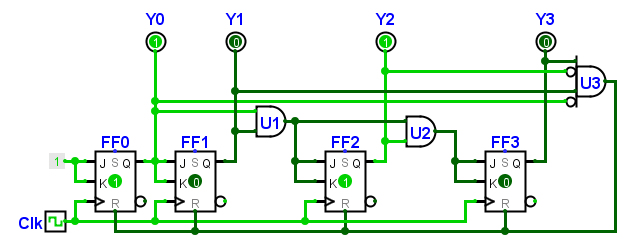
\includegraphics[width=\maxwidth{.95\linewidth}]{gfx/09_19}
	\caption{Decade Counter}
	\label{fig:09_19}
\end{figure}

This is only a four-bit counter (found in Figure \ref{fig:09_15}) but with an additional \textsf{AND} gate (\emph{U3}). The inputs for that \textsf{AND} gate are set such that when \emph{Y0}-\emph{Y3} are $ 1010 $ then the gate will activate and reset all four flip-flops.

Figure \ref{tmg:09_12} is the timing diagram obtained from the decade counter illustrated in Figure \ref{fig:09_19}.

\begin{figure}[H]
	\centering
	\begin{tikztimingtable}[
		timing/slope=0,         % no slope
		timing/coldist=2pt,     % column distance
		xscale=1.0,yscale=1.0,  % scale diagrams
		semithick,               % set line width
		]
		\footnotesize \# & U     R 18{2Q} 2U     \\
		\footnotesize Clk & 36{C} \\
		%                      P 01 02 03 04 05 06 07 08 09 10 11 12 13 14 15 16
	 %17 18
		\footnotesize Y0 & [] {L HH LL HH LL HH LL HH LL HH LL HH LL HH LL HH LL HH LL} \\
		\footnotesize Y1 & [] {L LL HH HH LL LL HH HH LL LL LL HH HH LL LL HH HH LL LL} \\
		\footnotesize Y2 & [] {L LL LL LL HH HH HH HH LL LL LL LL LL HH HH HH HH LL LL} \\
		\footnotesize Y3 & [] {L LL LL LL LL LL LL LL HH HH LL LL LL LL LL LL LL HH HH} \\
		\extracode % Optional
		% \fulltablegrid[]
		\vertlines[]{19}
		\tablerules[]
	\end{tikztimingtable}
	\caption{4-Bit Decade Counter Timing Diagram} 
	\label{tmg:09_12}
\end{figure}

The timing diagram shows the count increasing with each clock pulse (for example, at $ 8 $ the outputs are $ 1000 $) until pulse number ten, when the bits reset to $ 0000 $ and the count starts over. A vertical line was added at count ten for reference.

\subsection{Up-Down Counters}
\label{SL:subsec:up_down_counters}

In this chapter both up and down counters have been considered; however counters can also be designed to count both up and down. These counters are, of course, more complex than the simple counters encountered so far and Figure \ref{fig:09_20} illustrates an up-down counter circuit.

\begin{figure}[H]
	\centering
	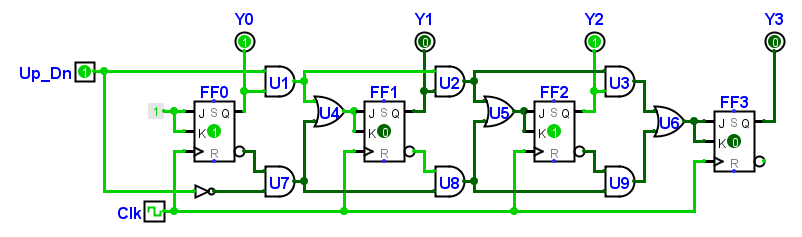
\includegraphics[width=\maxwidth{.95\linewidth}]{gfx/09_20}
	\caption{Up-Down Counter}
	\label{fig:09_20}
\end{figure}

When the \emph{Up\_Dn} bit is high the counter counts up but when that bit is low then the counter counts down. This counter is little more than a merging of the up counter in Figure \ref{fig:09_15} and the down counter in Figure \ref{fig:09_16}. \emph{U1}-\emph{U3} transmit the \emph{Q} outputs from each flip-flop to the next stage while \emph{U7}-\emph{U9} transmit the \emph{Q'} outputs from each flip-flop to the next stage. The E bit activates one of those two banks of \textsf{AND} gates.

No timing diagram is provided for this circuit since that diagram would be the same as for the up counter (Figure \ref{tmg:09_08} or the down counter (Figure \ref{tmg:09_09}), depending on the setting of the \emph{Up\_Dn} bit.

\subsection{Frequency Divider}
\label{SL:subsec:frequency_divider}

Often, a designer creates a system that may need various clock frequencies throughout its subsystems. In this case, it is desirable to have only one main pulse generator, but divide the frequency from that generator so other frequencies are available where they are needed. Also, by using a common clock source all of the frequencies are easier to synchronize when needed.

The circuit illustrated in Figure \ref{fig:09_21} is the same synchronous two-bit counter first considered in Figure \ref{fig:09_13}.

\begin{figure}[H]
	\centering
	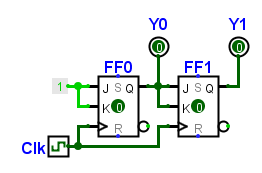
\includegraphics[width=\maxwidth{.95\linewidth}]{gfx/09_21}
	\caption{Synchronous 2-Bit Counter}
	\label{fig:09_21}
\end{figure}

The circuit in Figure \ref{fig:09_21} produces the timing diagram seen in Figure \ref{tmg:09_13}
 
\begin{figure}[H]
  \centering
  \begin{tikztimingtable}[
    timing/slope=0,         % no slope
    timing/coldist=2pt,     % column distance
    xscale=2.0,yscale=1.0,  % scale diagrams
    semithick,               % set line width
    ]
    \footnotesize \# & U     R 8{2Q} 2U     \\
    \footnotesize Clk & 17{C} \\
    %                 P 01 02 03 04 05 06 07 08
    \footnotesize Y0 & [] {L HH LL HH LL HH LL HH LL} \\
    \footnotesize Y1 & [] {L HH HH LL LL HH HH LL LL} \\
    \extracode % Optional
    % \fulltablegrid[]
    % \vertlines[]{}
    \tablerules[]
  \end{tikztimingtable}
  \caption{Frequency Divider} 
  \label{tmg:09_13}
\end{figure}

Notice that \emph{Y0} is half of the clock's frequency and \emph{Y1} is one-quarter of the clock's frequency. If the circuit designer used Y1 as a timer for some subcircuit then that circuit would operate at one-quarter of the main clock frequency. It is possible to use only one output port from a modulus counter, like the decade counter found in Figure \ref{fig:09_19}, and get any sort of division of the main clock desired.

\subsection{Counter Integrated Circuits (IC)}
\label{SL:subsec:counter_integrated_circuits}

In practice, most designers do not build counter circuits since there are so many types already commercially available. When a counter is needed, a designer can select an appropriate counter from those available on the market. Here are just a few as examples of what is available: 

\begin{table}[H]
  \sffamily
  \newcommand{\head}[1]{\textcolor{white}{\textbf{#1}}}    
  \begin{center}
    \rowcolors{2}{gray!10}{white} % Color every other line a light gray
    \begin{tabular}{ll} 
      \rowcolor{black!75}
      \head{IC} & \head{Function} \\
      74x68 & dual four-bit decade counter \\
      74x69 & dual four-bit binary counter \\
      74x90 & decade counter (divide by $ 2 $ and divide by $ 5 $ sections) \\
      74x143 & decade counter/latch/decoder/seven-segment driver \\
      74x163 & synchronous four-bit binary counter \\
      74x168 & synchronous four-bit up/down decade counter \\
      74x177 & presettable binary counter/latch \\
      74x291 & four-bit universal shift register and up/down counter
    \end{tabular}
  \end{center}
  \caption{Counter IC's}
  \label{sl:tab:counter_ics}
\end{table}

\section{Memory}
\label{SL:sec:memory}

\subsection{Read-Only Memory}
\label{SL:subsec:read-only_memory}

\acf{ROM} is an \ac{IC} that contains tens-of-millions of registers (memory locations) to store information. Typically, \ac{ROM} stores microcode (like bootup routines) and computer settings that do not change. There are several types of \ac{ROM}: mask, programmable, and erasable. 

\begin{itemize}
  \item \textsc{Mask} \acp{ROM} are manufactured such that memory locations already filled with data and that cannot be altered by the end user. They are called ``mask'' \acp{ROM} since the manufacturing process includes applying a mask to the circuit as it is being created. 
  \item \textsc{\acp{PROM}} are a type of \ac{ROM} that can be programmed by the end user, but it cannot be altered after that initial programming. This permits a designer to distribute some sort of program on a chip that is designed to be installed in some device and then never changed.
  \item \textsc{Erasable \acp{PROM}} can be programmed by the end user and then be later altered. An example of where an erasable \ac{PROM} would be used is in a computer's \ac{BIOS} (the operating system that boots up a computer), where the user can alter certain ``persistent'' computer specifications, like the device boot order. 
\end{itemize}

Two major differences between \ac{ROM} and \ac{RAM} are 1) \ac{ROM}'s ability to hold data when the computer is powered off and 2) altering the data in \ac{RAM} is much faster than in an erasable \ac{PROM}.

\subsection{Random Access Memory}
\label{SL:subsec:random_access_memory}

\acf{RAM} is an integrated circuit that contains tens-of-millions of registers (memory locations) to store information. The \ac{RAM} \ac{IC} is designed to quickly store data found at its input port and then look-up and return stored data requested by the circuit. In a computer operation, \ac{RAM} contains both program code and user input (for example, the \emph{LibreOffice Writer} program along with whatever document the user is working on). There are two types of \ac{RAM}: dynamic and static. \ac{DRAM} stores bits in such a way that it must be ``refreshed'' (or ``strobed'') every few milliseconds. \ac{SRAM} uses flip-flops to store data so it does not need to be refreshed. One enhancement to \acp{DRAM} was to package several in a single \ac{IC} and then synchronize them so they act like a single larger memory; these are called \acp{SDRAM} and they are very popular for camera and cell phone memory.

Both \ac{ROM} and \ac{RAM} circuits use registers, flip-flops, and other components already considered in this chapter, but by the millions rather than just four or so at a time. There are no example circuits or timing diagrams for these devices in this book; however, the lab manual that accompanies this book includes activities for both \ac{ROM} and \ac{RAM} devices.

















